\documentclass[12pt, letterpaper, twoside]{article}

\usepackage{geometry}
\usepackage{graphicx}
\usepackage{amsmath, amsfonts, amssymb, bbm}
%\usepackage{lipsum}
\usepackage{fancyhdr}
%\usepackage{layout}
\usepackage{lettrine}
\usepackage[explicit]{titlesec}
\usepackage{hyperref}
\usepackage{watermark}
\usepackage{color}

%%%%%%%%%%%%%%%%%%%%%%%% 
% FONT SELECTION  
%%%%%%%%%%%%%%%%%%%%%%%% 

\usepackage[light]{iwona}
\usepackage[T1]{fontenc}

%%%%%%%%%%%%%%%%%%%%%%%%
% DEFINE COLORS
%%%%%%%%%%%%%%%%%%%%%%%%

\definecolor{grey}{rgb}{0.5,0.5,0.5}
\definecolor{l-grey}{rgb}{0.8,0.8,0.8}
\definecolor{withe}{rgb}{1,1,1}
\definecolor{black}{rgb}{0,0,0}

%%%%%%%%%%%%%%%%%%%%%%%% 
% PAGE LAYOUT
%%%%%%%%%%%%%%%%%%%%%%%%

% Paper Width 614pt
% Text fill symemetric 604pt
% Paper Height 794pt

\setlength{\voffset}{-0.5in}
\setlength{\hoffset}{-1in}
\setlength{\oddsidemargin}{65pt}
\setlength{\evensidemargin}{45pt}
\setlength{\topmargin}{0in}
\setlength{\headheight}{15pt}
\setlength{\headsep}{20pt}
\setlength{\marginparwidth}{0in}
\setlength{\marginparsep}{0in}
\setlength{\textheight}{635pt}
\setlength{\textwidth}{494pt}
\setlength{\footskip}{50pt}

%%%%%%%%%%%%%%%%%%%%%%%%
% TITLES LAYOUT
%%%%%%%%%%%%%%%%%%%%%%%%

\titleformat{\section}[display]
{\vspace*{150pt}
\bf\Huge}
{\begin{picture}(0,0)\put(-60,-30){\textcolor{grey}{\thesection}}\end{picture}}
{0pt}
{#1}
[]
\titlespacing*{\section}{40pt}{10pt}{40pt}[40pt]
\newcommand{\sectionbreak}{\cleardoublepage}


%%%%%%%%%%%%%%%%%%%%%%%%
% MATH OPERATORS AND 
% CUSTOM ENVIRONMENTS
%%%%%%%%%%%%%%%%%%%%%%%%
\DeclareMathOperator{\Tr}{Tr}
\DeclareMathOperator*{\Cov}{Cov}
\DeclareMathOperator{\cov}{Cov} 
  
\newcounter{observ}
\newenvironment{observ}{\refstepcounter{observ}
   \textit{\textbf{Observation \theobserv:}} \rmfamily}
     
\newenvironment{proof}{\textit{Proof:} \rmfamily}{\hfill$\square$}

\newcommand{\ket}[1]{\ensuremath{\vert #1 \rangle}}
\newcommand{\bra}[1]{\ensuremath{\langle #1 \vert}} 
\newcommand{\braket}[2]{\ensuremath{\langle #1 \vert #2 \rangle}} 
\newcommand{\braOket}[3]{\ensuremath{\langle #1 \vert #2 \vert #3 \rangle}}
\newcommand{\ketbra}[2]{\ensuremath{\vert #1 \rangle \! \langle #2 \vert}}
\newcommand{\meanO}[1]{\ensuremath{\langle #1 \rangle}}
\newcommand{\ver}[2]{\ensuremath{\genfrac{}{}{0pt}{}{#1}{#2}}}
\newcommand{\tr}[1]{\ensuremath{\Tr \lcua #1\rcua}}
\newcommand{\trsub}[2]{\ensuremath{\Tr_{#1} \lcua #2 \rcua }}
\newcommand{\bsym}[1]{\ensuremath{\boldsymbol{#1}}}

\def\be{\begin{equation}}
\def\ee{\end{equation}}
\def\bea{\begin{eqnarray}}
\def\eea{\end{eqnarray}}
\def\bse{\begin{subequations}} 
\def\ese{\end{subequations}}
\def\mtxid{\mathbbm{1}}
\def\lpar{\left(} 
\def\rpar{\right)}
\def\lcua{\left[}
\def\rcua{\right]}
\def\lcor{\left\{}
\def\rcor{\right\}}
\def\lang{\left\langle}
\def\rang{\right\rangle}
\def\l{\left} 
\def\r{\right}
\def\nnnl{\nonumber\\}
\def\nnnlq{\nonumber\\ && \quad}
\def\nnnlqq{\nonumber\\ && \qquad}
\def\nnnlqqq{\nonumber\\ && \quad\qquad}
\def\ie{, \textit{i.e.}, }

%%%%%%%%%%%%%%%%%%%%%%%%
% DOCUMENT
%%%%%%%%%%%%%%%%%%%%%%%%

\begin{document}


\pagestyle{fancy}
\renewcommand{\headrulewidth}{0pt}
\fancyhead{}
\fancyfoot{}

%%%%%%%%%%%%%%%%%%%%%%%%
% TITLE PAGE 
%%%%%%%%%%%%%%%%%%%%%%%%

%!TEX root = main.tex 

\thiswatermark{\centering
\put(0,-110){
\includegraphics[height=2.5cm]{img/0-Ztf.png}} 
\put(430,-100){
\includegraphics[height=2cm]{img/0-Ehu.png}}
} 

\begin{center}

\vspace*{20pt}
\textsc{\LARGE University of the Basque Country}

\vspace{20pt}
\textsc{\Large PhD Thesis}

\vspace{50pt} 
\hrule 

\vspace{16pt}
{\huge \bfseries Lower bounds on quantum metrological precisions}
\vspace{16pt}

\hrule
\vspace{40pt}

\begin{minipage}{0.4\textwidth}
\begin{flushleft} \large
\emph{Author:}


M. Sc. Iagoba \textsc{Apellaniz}
\end{flushleft}
\end{minipage}
\begin{minipage}{0.4\textwidth}
\begin{flushright} \large
\emph{Director:}

Prof. G\'eza \textsc{T\'oth} %TODO: Check Geza's name
\end{flushright}
\end{minipage}

\vspace{40pt}
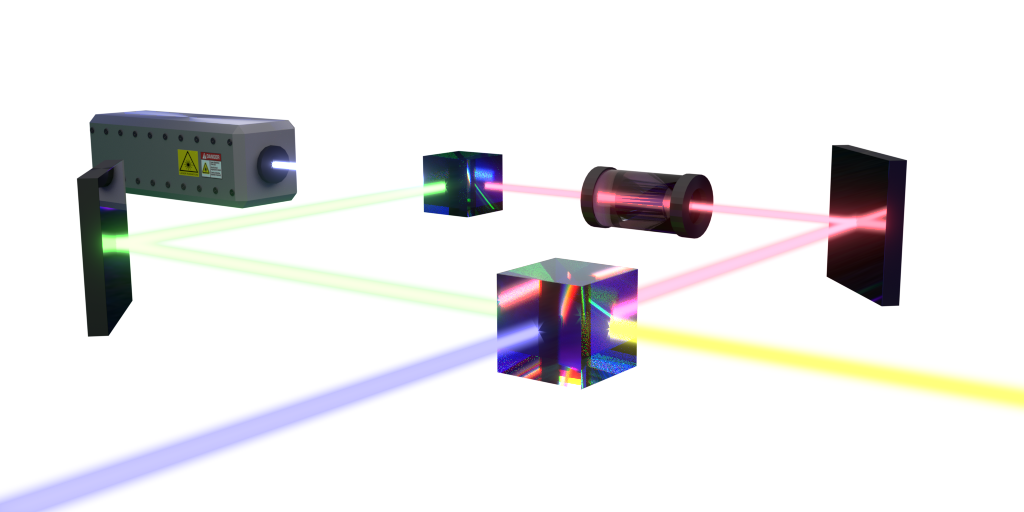
\includegraphics[width=0.8\hsize]{img/cover3Dpicture.png}
\vfill

% Bottom of the page
{\large \today}

\end{center}

\cleardoublepage

%%%%%%%%%%%%%%%%%%%%%%%%
% EDITION TIPS
%%%%%%%%%%%%%%%%%%%%%%%%

\cleardoublepage

This document was generated with the 2014 distribution of \LaTeX. 

\vfill


\includegraphics[height=20pt]{img/0-CreativeCommons-by-sa.png}

2012-2015 Iagoba Apellaniz. This work is licensed under the Creative Commons
Attribution-ShareAlike 4.0 International License. To view a copy of this
license, visit
\href{http://creativecommons.org/licenses/by-sa/4.0/deed.en_US}
{http://creativecommons.org/ licenses/by-sa/4.0/deed.en\_US}.
\clearpage

%%%%%%%%%%%%%%%%%%%%%%%%
% PROLOGE
%%%%%%%%%%%%%%%%%%%%%%%%

\section*{Prologue}
\setcounter{page}{1}
\pagenumbering{roman}
\fancyfoot[LE,RO]{\thepage}

\lettrine[lines=2, findent=3pt,nindent=0pt]{T}{his} work is part of the doctoral project on Quantum Information which I started on the sumer of 2013.
This work collects part of the research I have done on these previous years.
I will try to be clear throughout all the thesis such that make it readable for a wider audience as it is possible.
This way I hope it will be readable by any person with a bachelor in science, particularly in physics or at least with a partial knowledge in Quantum Mechanics.
With that in mind the first and the second chapters will be used to introduce the reader into the context on which this thesis was written as well as the basic notions of Quantum Metrology, the enveloping field of the present work.
Even though I write this thesis for a broad audience in mind, a basic notion on quantum physics and statistics is needed to follow it properly as I said before.
For instance, I will assume among other things that the reader knows what probability is and which are its properties, or what a quantum state is and what it represents.
I will give references where to find such complementary material when I think is necessary.

This research I publish in a thesis form is part of the work done within the Research Group in Quantum Information in which Prof.
G\'eza T\'oth is the group leader and principal investigator.
I have to mentions the rest of the members of the group Dr. Philipp Hyllus, Dr. Giuseppe Vitagliano, Dr. I\~nigo Urizar-Lanz, Dr. Zolt\'an Zinbor\'as and Dr. Matthias Kleinmann at the time I was working on the projects of this thesis.
Some of them may still be part of the group and some not.
Apart from the group of G\'eza T\'oth based in Bilbao, Spain, this thesis also collects some work done in collaboration with the Theoretical Quantum Optics (TQO) group lead by Prof. Otfried G\"uhne at the University of Siegen, Germany, and the group of Prof. Carsten Klempt at the Leibniz University in Hannover, based also in Germany.
The last one is an experimental group specialized on the creation of exotic quantum states with very many particles with a variety of applications in quantum technology.

First, we investigate the metrological usefulness of a family of states known as the unpolarized Dicke states, which have boosted the sensitivity of magnetometry when lots of particles are used in the sense that quantum enhancements play a very important role to achieve such a precision.
Second, we investigate possible lower bounds on the quantum Fisher information, a quantity that characterizes the usefulness of a state for quantum metrology, using the theory of Legendre transforms such that we obtain thight lower bounds based on few measurements of the initial quantum state that will be used for metrology.
And last but not least, we investigate the gradient magnetometry, i.e., we develop a theory to study the capablilities of some states to sense the change in space of the magnetic field and we apply that theory to some known states.

Before the thesis work the reader can find the present prologue, the list of publications, the table of contents, and a list of abbreviations, figures and tables.
Then, the thesis starts.
On the first pages one can find a brief dedicatory and acknowledgements followed by the chapters.
The content of the chapters is organized as follows.
First, I start with an introduction to describe the current situation of Quantum Information spetially Quantum Metrology and I write about the basics of Quantum Metrology and how it emerges from statics and Quantum Mechanics.
Second, I present the reader our works in characterizing the family of states known as the unpolarized Dicke states, in optimizing the lower bound for the quantum Fisher information when some expectation values of the states are known and our work in gradient quantum metrology.

\begin{flushright}
  Iagoba Apellaniz

  Bilbao, \today
\end{flushright}


\section*{Publications}
{\setlength{\parindent}{0cm}
Iagoba Apellaniz \textit{et al} 2015 \textit{New J. Phys.} \textbf{17} 083027

Detecting metrologically useful entanglement in the vicinity of Dicke states

\subsection*{Preprints}
\subsection*{Out of the scope of this thesis}
G\'eza T\'oth and Iagoba Apellaniz 2014 \textit{J. Phys. A: Math. Theor.} \textbf{47} 424006

Quantum metrology from a quantum information science prespective
\vspace{10pt}

Giuseppe Vitagliano \textit{et al} 2014 \textit{Phys. Rev. A} \textbf{89} 032307

Spin squeezing and entanglement for an arbitrary spin
}
%%%%%%%%%%%%%%%%%%%%%%%%
% TABLE OF CONTENTS
%%%%%%%%%%%%%%%%%%%%%%%%

\vspace*{100pt}
\tableofcontents

%%%%%%%%%%%%%%%%%%%%%%%%
% FIGURES TABLES, ETC
%%%%%%%%%%%%%%%%%%%%%%%%
\section*{Tables, figures and abbreviations used in this book}
\fancyfoot[LE,RO]{\thepage}

[Insert in a table]

SLD - Symmetric logarithmic derivative.

qFI - Quantum Fisher information

%%%%%%%%%%%%%%%%%%%%%%%%
% THESIS
%%%%%%%%%%%%%%%%%%%%%%%%

\cleardoublepage

\pagenumbering{arabic}
\fancyfoot{}
%!TEX root = main.tex 

\thiswatermark{\centering
\put(0,-110){
\includegraphics[height=2.5cm]{img/0-Ztf.png}} 
\put(430,-100){
\includegraphics[height=2cm]{img/0-Ehu.png}}
} 

\begin{center}

\vspace*{20pt}
\textsc{\LARGE University of the Basque Country}

\vspace{20pt}
\textsc{\Large PhD Thesis}

\vspace{50pt} 
\hrule 

\vspace{16pt}
{\huge \bfseries Lower bounds on quantum metrological precisions}
\vspace{16pt}

\hrule
\vspace{40pt}

\begin{minipage}{0.4\textwidth}
\begin{flushleft} \large
\emph{Author:}


M. Sc. Iagoba \textsc{Apellaniz}
\end{flushleft}
\end{minipage}
\begin{minipage}{0.4\textwidth}
\begin{flushright} \large
\emph{Director:}

Prof. G\'eza \textsc{T\'oth} %TODO: Check Geza's name
\end{flushright}
\end{minipage}

\vspace{40pt}
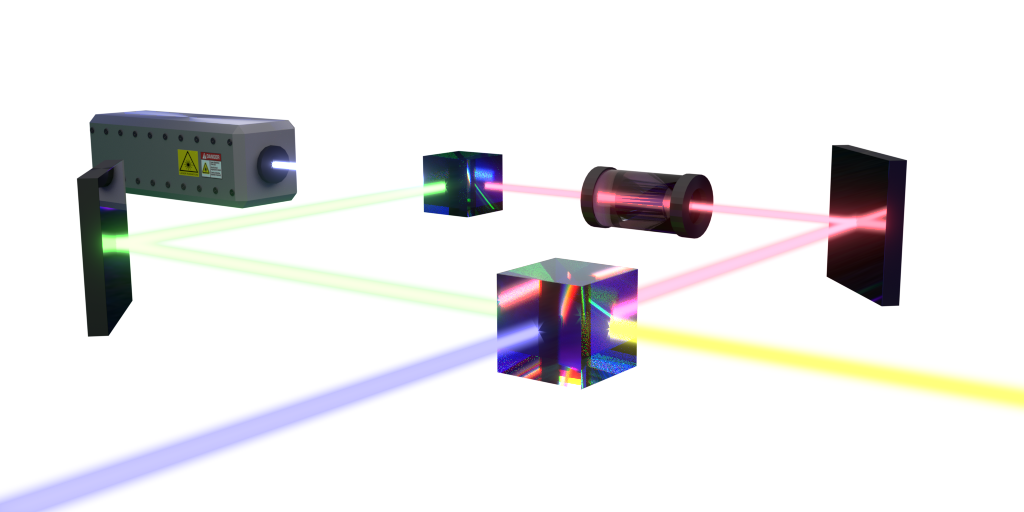
\includegraphics[width=0.8\hsize]{img/cover3Dpicture.png}
\vfill

% Bottom of the page
{\large \today}

\end{center}

\cleardoublepage
\cleardoublepage
\setcounter{page}{1}

%%%%%%%%%%%%%%%%%%%%%%%%
% DEDICATION PAGE
%%%%%%%%%%%%%%%%%%%%%%%%
\vspace*{100pt}
\begin{center}
\emph{To my parents and my family}
\end{center}

\cleardoublepage

%%%%%%%%%%%%%%%%%%%%%%%%
% HEADINGS AND PAGE NUM.
%%%%%%%%%%%%%%%%%%%%%%%%

\renewcommand{\rightmark}{\bf \thesubsection}
\renewcommand{\headrulewidth}{0.5pt}
\fancyfoot[LE,RO]{\thepage}
\fancyhead[LE]{Section: \rightmark} % TODO: Solve heading
\fancyhead[RO]{\leftmark}

%%%%%%%%%%%%%%%%%%%%%%%%
% REDEFINE TITLE FORMAT
%%%%%%%%%%%%%%%%%%%%%%%%
\titleformat{\section}[display]
{\vspace*{190pt}
\bf\Huge}
{\begin{picture}(0,0)\put(-64,-31){\textcolor{grey}{\thesection}}\end{picture}}
{0pt}
{\textcolor{withe}{#1}}
[]
\titlespacing*{\section}{100pt}{10pt}{40pt}[40pt]


\section{Introduction}
\thiswatermark{\put(1,-297){\color{l-grey}\rule{84pt}{42pt}}
\put(84,-297){\color{grey}\rule{410pt}{42pt}}}

%!TEX root = main.tex

% Section: Introduction
\lettrine[lines=2, findent=3pt,nindent=0pt]{M}{etrology} has played an inportant role since [TODO: add historical reasons]. With the development of quantum technology, a more deep understanding of one of its aspect as the quantum metrology is needed. Therefore, many works appeared recently on the literature. 

In this work the author, in collaboration with other researchers [TODO: see how to add reference to the rest of collavorators], has addressed some crucial questions regarding this field. 


\section{Background on Estimation and on Quantum Information Theories}
\thiswatermark{\put(1,-327){\color{l-grey}\rule{84pt}{72pt}}
\put(84,-327){\color{grey}\rule{410pt}{72pt}}}

\lettrine[lines=2, findent=3pt,nindent=0pt]{T}{his} thesis is based on
many previous works developed since long time ago.
It is known that estimation processes are part of different
aspects of the human been behaviour.
From the estimation of the season on which one has 
to plant some vegetables to grow until the estimation of which route is the
shorter to reach somewhere. 
All these processes usually involve a huge amount of data. 
So it has been developed a strongly consolidated theory around that.

Hello thi is where sample text was. 

\subsection{Classical estimation theory}
Hello thi is where sample text was.

\subsection{Step in quantum estimation theory}
Hello thi is where sample text was.

\subsection{Quantum Metrology}
Hello thi is where sample text was.

\section{Quantum metrology with Dicke like states}
\thiswatermark{\put(1,-327){\color{l-grey}\rule{84pt}{72pt}}
\put(84,-327){\color{grey}\rule{410pt}{72pt}}} 
Hello thi is where sample text was.

\section[Bounding qFI with observables]
{Bounding quantum Fisher \qquad\qquad\, Information with observables}
\thiswatermark{\put(1,-327){\color{l-grey}\rule{84pt}{72pt}}
\put(84,-327){\color{grey}\rule{410pt}{72pt}}} 
Hello thi is where sample text was.

\section{Accuracy bound for gradient field estimation with atomic ensembles}
\thiswatermark{\put(1,-327){\color{l-grey}\rule{84pt}{72pt}}
\put(84,-327){\color{grey}\rule{410pt}{72pt}}} 
Hello thi is where sample text was.

%%%%%%%%%%%%%%%%%%%%%%%%
% REDEFINE TITLE FORMAT
%%%%%%%%%%%%%%%%%%%%%%%%
\titleformat{\section}[display]
{\vspace*{150pt}
\bf\Huge}
{\begin{picture}(0,0)\put(-60,-30){\textcolor{grey}{\thesection}}\end{picture}}
{0pt}
{#1}
[]
\titlespacing*{\section}{40pt}{10pt}{40pt}[40pt]

\section*{References}
Hello thi is where sample text was.

\section*{Index}
Hello thi is where sample text was.

\end{document}
